\begin{document}
\begin{figure}[htbp]
\centering
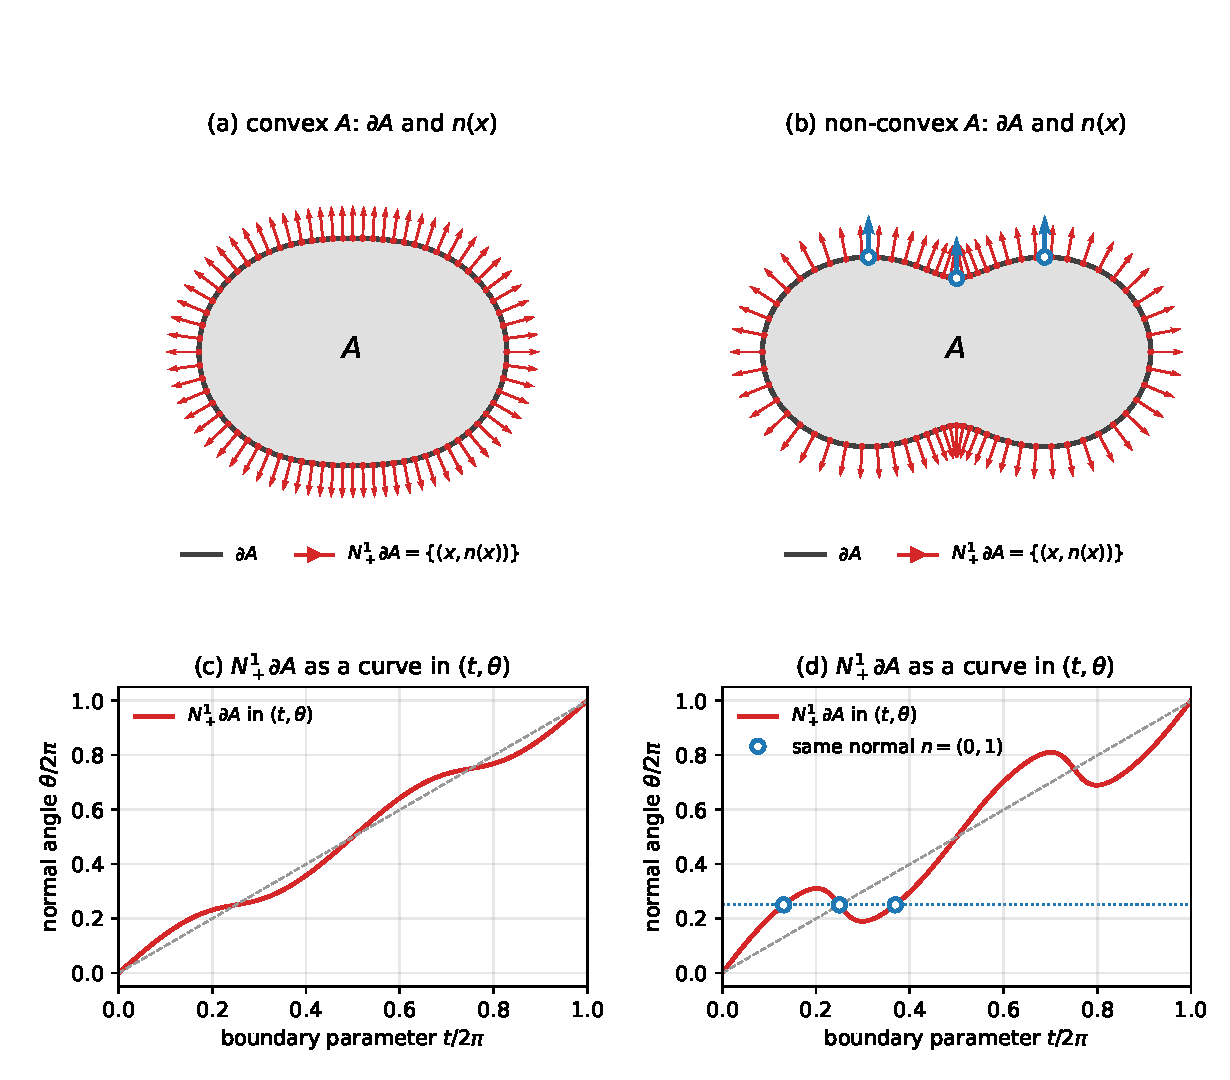
\includegraphics[width=0.74\textwidth]{fig_normal_bundle.pdf}
\caption{Outward unit normal bundles in the plane. (a),(b): a strictly convex set and a non-convex set $A$ (shaded),
with the boundary $\partial A$ (dark grey) and the outward unit normal $n(x)\in\Sph^1$ drawn at a sample of boundary
points. Everything in red is $\Nb$: the set of all pairs $(x,n(x))$, a closed curve in $\R^2\times\Sph^1$ whose
front is $\partial A$. (c),(d): the same curve $\Nb$ drawn in coordinates $(t,\theta)$, where $t$ parametrises
$\partial A$ and $\theta$ is the angle of $n(x(t))$. For the convex set the angle is monotone,
so $x\mapsto n(x)$ is a bijection $\partial A\to\Sph^1$ and $\Nb$ is a graph over $\Sph^1$; this is the setting of
the boundary map~\eqref{eq:boundary-map}. For the non-convex set the same normal direction occurs at several boundary
points, and $\Nb$ is no longer a graph over $\Sph^1$: the three blue points in (b) all have normal $n=(0,1)$, and in
(d) they are the three intersections of $\Nb$ with the level line $\theta=\pi/2$ (dotted).}
\label{fig:normal-bundle}
\end{figure}

\paragraph{Convexity.}


We begin by considering a linear contraction, where in this specific case it can be shown that the attractor is convex \note{ref Tei, Lamb linear map here}, and that the boundary of the attractor is smooth. This is a consequence of the linear contractive dynamics, but more generally we can loosen these constraints \note{ref Kourliouros normal hyperbol -> thm 1.2}.  

\paragraph{The dual picture: support functions.}


Convexity is a statement about the other projection of $\Nb$, namely $(x,n)\mapsto n$. If $A$ is strictly convex,
every local normal $n(x)$, the annihilator of $T_x\partial A$, is also a global supporting covector, the Gauss map
$x\mapsto n(x)$ is a bijection $\partial A\to\Sph^{d-1}$, and $\partial A$ is recovered from the support function
$h_A(n)=\max_{y\in A}\langle n,y\rangle$ as $x(n)=\nabla h_A(n)$. When convexity fails the lift $\Nb$ is still a
smooth Legendrian, but its projection to $\Sph^{d-1}$ folds where the Gauss curvature $\det Dn_x$ vanishes. In the
dual coordinates $(n,\langle n,x\rangle)$ the lift then traces a swallowtail (\cref{fig:support}): $h_A=h_{\operatorname{conv}A}$
is its upper envelope, it is not differentiable in directions supported at two points, and the normals along the
dented part of $\partial A$ remain annihilators of tangent spaces without being supporting covectors. The set-valued
map $F_{f,\eps}$ only sees such outer envelopes, while $\beta_{f,\eps}$ keeps every Legendrian lift smooth; this
selection step is one mechanism by which corners can appear on perturbed boundaries.

\begin{figure}[htbp]
\centering
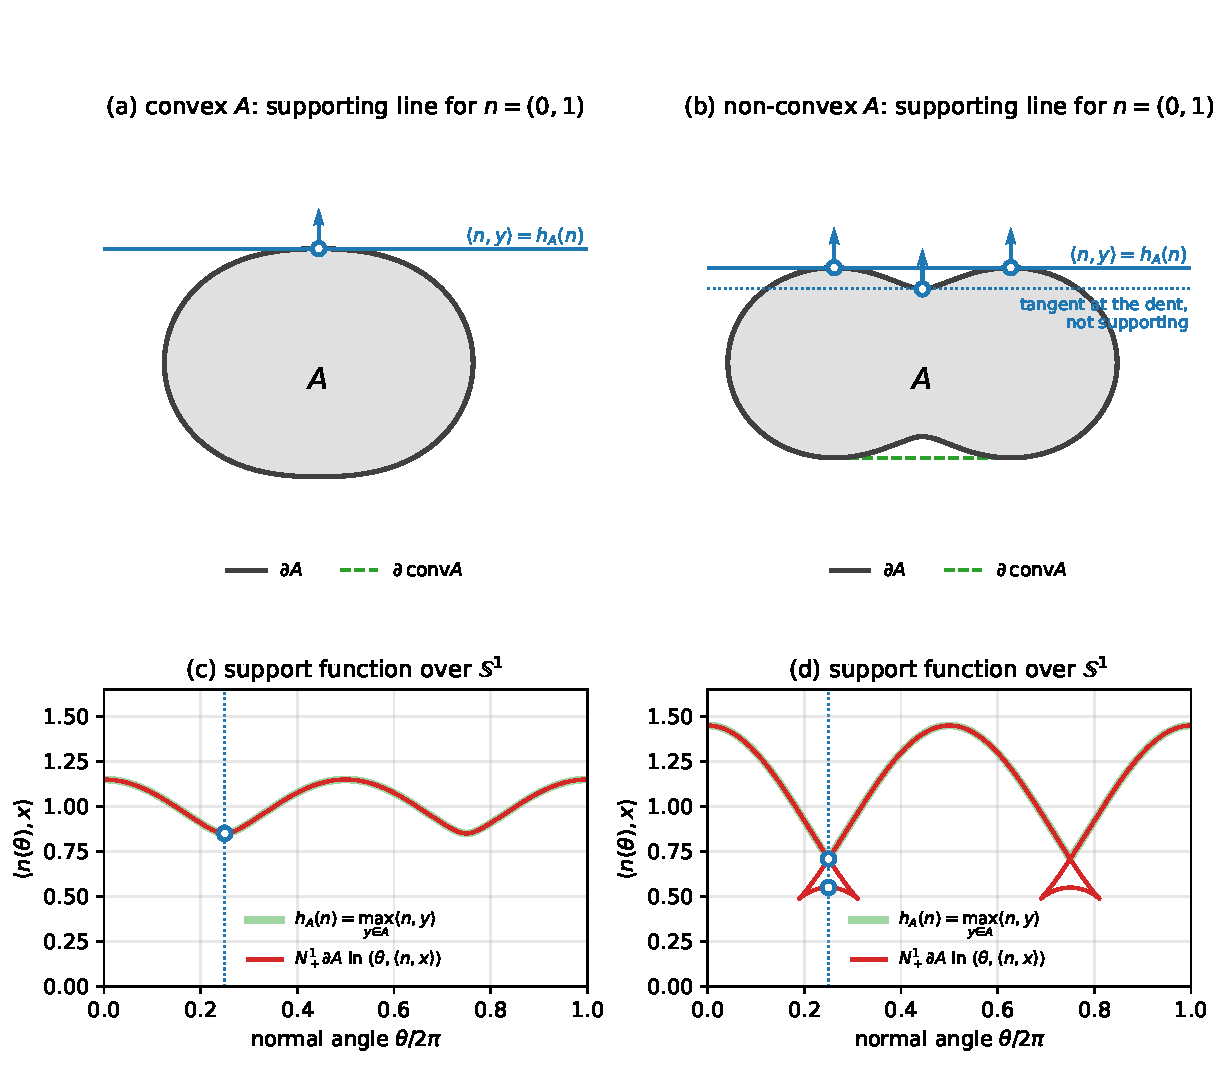
\includegraphics[width=0.74\textwidth]{fig_support_function.pdf}
\caption{The Legendre-dual picture of \cref{fig:normal-bundle}. (a),(b): the sets $A$ with their convex hull
(dashed green, differing from $\partial A$ only across the dents) and the supporting line $\langle n,y\rangle=h_A(n)$
for $n=(0,1)$ (blue). For the convex set it touches $\partial A$ at one point. For the non-convex set it touches at
the two humps, while the tangent line at the dent point, which has the same local normal, cuts through $A$ (dotted).
(c),(d): $\Nb$ projected to $(\theta,\langle n,x\rangle)$, the multivalued support function (red), and the true support
function $h_A$ (green). For the convex set the two coincide. For the non-convex set the red curve is a swallowtail
with cusps at the zero-curvature points of $\partial A$; $h_A$ is its upper envelope, with a corner at $\theta=\pi/2$
where the two hump points give the same value, and the dent point lies on the discarded lower branch.}
\label{fig:support}
\end{figure}

\paragraph{Contact viewpoint.}
$\R^d\times\Sph^{d-1}$ carries the contact form $\alpha = n\cdot dx$. Unit normal bundles of hypersurfaces are
Legendrian, and $\beta_{f,\eps}$ is a (conformal) contactomorphism (\cref{lem:contact}). Boundary maps are thus among
the simplest non-trivial contactomorphisms. Their invariant Legendrian submanifolds and the projections of these to
$\R^d$ (\emph{fronts}) can be expected to show, at least locally, behaviour that general contactomorphisms exhibit.


\begin{enumerate}[label=\textbf{(\Alph*)},leftmargin=*]
  \item \textbf{Linear contact algebra.} Linear symplectic algebra constrains the spectra of symplectic maps
  ($\nu\leftrightarrow1/\nu$) and organises their normal forms and bifurcations (Krein collisions). The analogous
  question for contactomorphisms is which geometry the contact structure forces on the linearisation at fixed and
  periodic points, and how much of the singularity picture it predicts.
  \item \textbf{Pontryagin flows and control.} The set-valued map $F_{f,\eps}$ is a control system
  $x_{i+1}=f(x_i)+u_i$, $\|u_i\|\le\eps$, whose attractor is a reachable set. The boundary map is the spherised
  extremal map of Pontryagin's maximum principle. This links attractor boundaries to the geometric theory of optimal
  control and reachable sets.
\end{enumerate}

This report gives background (\cref{sec:background}), presents preliminary results for the linear diagonal case,
which settle Task~1 and illustrate both strands (\cref{sec:results}), and describes the plan (\cref{sec:plan}).

\end{document}
